%To compile as handout, use
%pdflatex "\def\ishandout{1} \input{filename.tex}"
%Defaults to non-handout mode (with slide reveals)
\ifdefined\ishandout
  \documentclass[handout]{beamer}
\else
  \documentclass{beamer}
\fi
 
\usepackage{econ103slides} 

\date{Lecture 21}


\begin{document} 




%%%%%%%%%%%%%%%%%%%%%%%%%%%%%%%%%%%%%%%%

\begin{frame}[plain]
	\titlepage 
	

\end{frame} 

%%%%%%%%%%%%%%%%%%%%%%%%%%%%%%%%%%%%%%%%
\begin{frame}
\begin{center}
\Huge Hypothesis Testing III
\end{center}
\end{frame}

%%%%%%%%%%%%%%%%%%%%%%%%%%%%%%%%%%%%%%%%
\begin{frame}
\begin{block}
	{Last Time}
	Walked through steps of hypothesis testing in a simple example.
\end{block}
\begin{alertblock}
	{Today}
	\begin{itemize}
		\item Relationship between hypothesis testing and CIs
		\item More examples of hypothesis tests
	\end{itemize}
\end{alertblock}
\end{frame}


%%%%%%%%%%%%%%%%%%%%%%%%%%%%%%%%%%%%%%%%
\begin{frame}
	\frametitle{Relationship between CI and Two-Sided Test}

	\begin{itemize}
		\item There is a \emph{very close} relationship between CIs and hypothesis tests against a two-sided alternative.
		\item I'll illustrate this using a generic version of the example from last class but the relationship holds \emph{in general}.
	\end{itemize}
\end{frame}
%%%%%%%%%%%%%%%%%%%%%%%%%%%%%%%%%%%%%%%%
\begin{frame}
\frametitle{Relationship between CI and Two-sided Test}
Suppose $X_1, \hdots, X_n \sim \mbox{iid } N(\mu,\sigma^2)$

\vspace{1em}
	\begin{block}{Test $H_0\colon \mu = \mu_0$ vs.\ $H_1\colon \mu \neq \mu_0$ at significance level $\alpha$} 
		\begin{itemize}
			\item Test Statistic:  $T_n = \sqrt{n}(\bar{X}_n - \mu_0)/S \sim t(n-1)$ under $H_0$ 
			\item Decision Rule: Reject $H_0$ if $|T_n| > \texttt{qt}(1-\alpha/2, \texttt{df}=n-1)$ 
			\end{itemize}

			\pause
\end{block}
	\begin{block}{$100\times (1-\alpha)\%$ CI for $\mu$} 
		$$\bar{X}_n \pm \texttt{qt}(1-\alpha/2, \texttt{df}=n-1) \frac{S}{\sqrt{n}}$$
\end{block}
\end{frame}
%%%%%%%%%%%%%%%%%%%%%%%%%%%%%%%%%%%%%%%%
\begin{frame}
\frametitle{Relationship between CI and Two-sided Test}
$\alert{c =  \texttt{qt}(1-\alpha/2, \texttt{df}=n-1)}$
\begin{block}{Decision Rule: Reject $H_0$ if}
		$$\left|\frac{\bar{X}_n - \mu_0}{S/\sqrt{n}} \right|> c \quad \iff \pause  \quad \left(\frac{\bar{X}_n - \mu_0}{S/\sqrt{n}}> c \;\;\mbox{  \alert{OR}  }\;\;\frac{\bar{X}_n - \mu_0}{S/\sqrt{n}}< - c\right)$$
\end{block}

\pause
\begin{block}{Equivalent to: \emph{Don't Reject} $H_0$ provided}
	$$-c \leq \frac{\bar{X}_n - \mu_0}{S/\sqrt{n}}\leq c $$ \pause
	$$\alert{\bar{X_n} - c\times \frac{S}{\sqrt{n}} \leq \mu_0 \leq \bar{X_n} + c\times \frac{S}{\sqrt{n}}}$$
\end{block}
\end{frame}
%%%%%%%%%%%%%%%%%%%%%%%%%%%%%%%%%%%%%%%%
\begin{frame}
\frametitle{What does this mean?}

\begin{block}
	{Two-sided Test $\iff$ Checking if $\mu_0 \in$ CI}
	A two-sided test of $H_0\colon \mu = \mu_0$ against $H_1\colon \mu\neq \mu_0 $ at significance level $\alpha$ is equivalent to checking whether $\mu_0$ lies inside the corresponding $100\times (1-\alpha)\%$ confidence interval for $\mu$.
\end{block}

\pause

\begin{block}
	{``Inverting'' Two-sided Test to get a CI}	
	Collect all the values $\mu_0$ such that we cannot reject $H_0\colon \mu = \mu_0$ against the two-sided alternative. The result is \emph{precisely} a $100\times (1-\alpha)\%$ CI for $\mu$.
\end{block}
\end{frame}
%%%%%%%%%%%%%%%%%%%%%%%%%%%%%%%%%%%%%%%%
%%%%%%%%%%%%%%%%%%%%%%%%%%%%%%%%%%%%%%%%
\begin{frame}
\frametitle{The Anchoring Experiment}
\begin{figure}
\centering
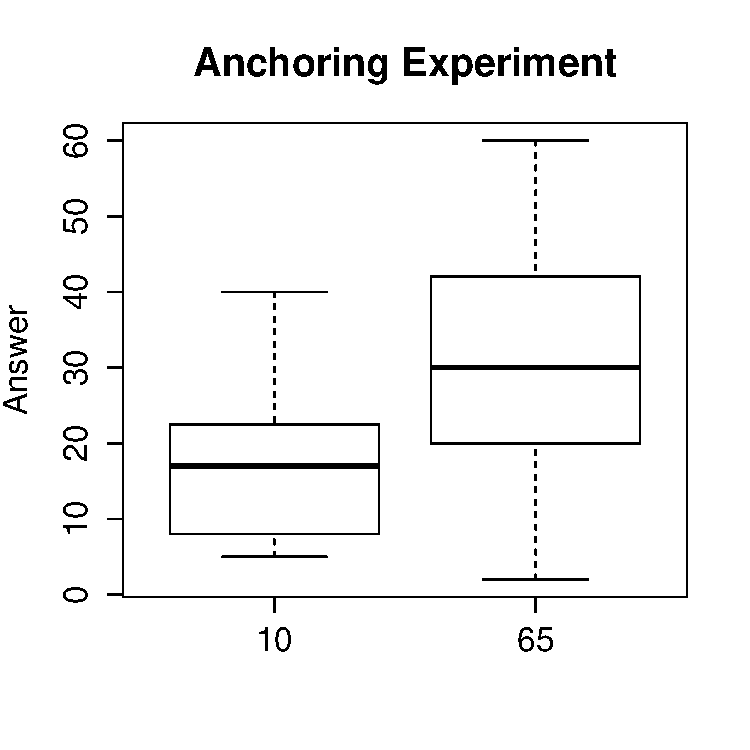
\includegraphics[scale = 0.55]{./images/anchoring_boxplot}
\end{figure}
\end{frame}
%%%%%%%%%%%%%%%%%%%%%%%%%%%%%%%%%%%%%%%%%
\begin{frame}
\frametitle{The Anchoring Experiment}
Shown a ``random'' number and then asked what proportion of UN member states are located in Africa.
	\begin{block}{``Hi'' Group -- Shown 65 ($n_{Hi}=46$)}
		Sample Mean: $30.7$, Sample Variance: $253$
\end{block}


	\begin{block}{``Lo'' Group -- Shown 10 ($n_{Lo}=43$)}
	Sample Mean: $17.1$, Sample Variance: $86$
\end{block}


\vspace{1em}

\hfill\alert{\fbox{Fairly large samples here, so we'll proceed via the CLT...}}
\end{frame}
%%%%%%%%%%%%%%%%%%%%%%%%%%%%%%%%%%%%%%%

\begin{frame}
	\frametitle{In words, what is our null hypothesis?\hfill 
\includegraphics[scale = 0.05]{./images/clicker}}

	\begin{enumerate}[(a)]
		\item There is a \emph{positive} anchoring effect: seeing a higher random number makes people report a higher answer.
		\item There is a \emph{negative} anchoring effect: seeing a lower random number makes people report a lower answer. 
		\item There \emph{is} an anchoring effect: it could be positive or negative.
		\item There is  \emph{no} anchoring effect: people aren't influenced by seeing a random number before answering.
	\end{enumerate}
\end{frame}
%%%%%%%%%%%%%%%%%%%%%%%%%%%%%%%%%%%%%%%
\begin{frame}
	\frametitle{In symbols, what is our null hypothesis?\hfill 
\includegraphics[scale = 0.05]{./images/clicker}}

	\begin{enumerate}[(a)]
		\item $\mu_{Lo} < \mu_{Hi}$
		\item $\mu_{Lo} = \mu_{Hi}$
		\item $\mu_{Lo} > \mu_{Hi}$
		\item $\mu_{Lo} \neq \mu_{Hi}$
	\end{enumerate}
\pause
	\vspace{1em}

	\alert{$\mu_{Lo} = \mu_{Hi}$ is \emph{equivalent to} $\mu_{Hi} - \mu_{Lo} = 0$!}
\end{frame}
%%%%%%%%%%%%%%%%%%%%%%%%%%%%%%%%%%%%%%%
\begin{frame}
	\frametitle{Anchoring Experiment\hfill 
\includegraphics[scale = 0.05]{./images/clicker}}
 
Under the null, what should we expect to be true about the values taken on by $\bar{X}_{Lo}$ and $\bar{X}_{Hi}$?

\vspace{1em}

	\begin{enumerate}[(a)]
		\item They should be similar in value.
		\item $\bar{X}_{Lo}$ should be the smaller of the two.
		\item $\bar{X}_{Hi}$ should be the smaller of the two.
		\item They should be different. We don't know which will be larger.
	\end{enumerate}
\end{frame}
%%%%%%%%%%%%%%%%%%%%%%%%%%%%%%%%%%%%%%%%

\begin{frame}
\frametitle{What is our Test Statistic?}
\begin{block}{Sampling Distribution}
		$$\frac{\left(\bar{X}_{Hi} - \bar{X}_{Lo}\right) - \left(\mu_{Hi} - \mu_{Lo}\right)}{\sqrt{\frac{S_{Hi}^2}{n_{Hi}} + \frac{S_{Lo}^2}{n_{Lo}}}} \approx N(0,1)$$
\end{block}

\begin{block}{Test Statistic: Impose the Null}
Under $H_0\colon \mu_{Lo} = \mu_{Hi}$
	$$T_n =\frac{\bar{X}_{Hi} - \bar{X}_{Lo}}{\sqrt{\frac{S_{Hi}^2}{n_{Hi}} + \frac{S_{Lo}^2}{n_{Lo}}}} \approx N(0,1)$$
\end{block}
\end{frame}


%%%%%%%%%%%%%%%%%%%%%%%%%%%%%%%%%%%%%%%%
\begin{frame}
\frametitle{What is our Test Statistic?}
\footnotesize
$\bar{X}_{Hi} = 30.7$, $s^2_{Hi} = 253$, $n_{Hi} = 46$\\
$\bar{X}_{Lo} = 17.1$, $s^2_{Lo} = 86$, $n_{Lo} = 43$\\
\normalsize
\vspace{2em}

\begin{block}{Under $H_0\colon \mu_{Lo} = \mu_{Hi}$}
	$$T_n = \frac{\bar{X}_{Hi} - \bar{X}_{Lo}}{\sqrt{\frac{S_{Hi}^2}{n_{Hi}} + \frac{S_{Lo}^2}{n_{Lo}}}} \approx N(0,1)$$
\end{block}

\begin{block}{Plugging in Our Data}
$$T_n = \frac{\bar{X}_{Hi} - \bar{X}_{Lo}}{\sqrt{\frac{S_{Hi}^2}{n_{Hi}} + \frac{S_{Lo}^2}{n_{Lo}}}} \approx 5$$
\end{block}
\end{frame}


%%%%%%%%%%%%%%%%%%%%%%%%%%%%%%%%%%%%%%%%
\begin{frame}[t]
\frametitle{Anchoring Experiment Example \hfill 
\includegraphics[scale = 0.05]{./images/clicker}}
Approximately what critical value should we use to test $H_0\colon \mu_{Lo} = \mu_{Hi}$ against the two-sided alternative at the 5\% significance level?

\pause
\vspace{1em}
\begin{center}
\begin{tabular}{l|lll}
$\alpha$ &   0.10& 0.05 &0.01\\
\hline
\texttt{qnorm($1-\alpha$)} & 1.28 &1.64 &2.33\\
\texttt{qnorm($1-\alpha/2$)} &1.64 &\alert{1.96}& 2.58
\end{tabular}
\end{center}
\hfill \alert{... Approximately 2}
\end{frame}
%%%%%%%%%%%%%%%%%%%%%%%%%%%%%%%%%%%%%%%%
\begin{frame}
\frametitle{Anchoring Experiment Example\hfill 
\includegraphics[scale = 0.05]{./images/clicker}}
Which of these commands would give us the p-value of our test of $H_0\colon \mu_{Lo} = \mu_{Hi}$ against $H_1\colon \mu_{Lo}<\mu_{Hi}$ at significance level $\alpha$?
\vspace{1em}
	\begin{enumerate}[(a)]
		\item \texttt{qnorm($1-\alpha$)}
		\item \texttt{qnorm($1-\alpha/2$)}
		\item \texttt{1 - pnorm(5)}
		\item \texttt{2 * (1 - pnorm(5))}
	\end{enumerate}
	

\end{frame}
%%%%%%%%%%%%%%%%%%%%%%%%%%%%%%%%%%%%%%%%

\begin{frame}
\frametitle{P-values for $H_0\colon \mu_{Lo} = \mu_{Hi}$}
We plug in the value of the test statistic that we observed: 5
\begin{block}{Against $H_1\colon \mu_{Lo}< \mu_{Hi}$}
\texttt{1 - pnorm(5)} $< 0.0000$
\end{block}

\begin{block}{Against $H_1\colon \mu_{Lo}\neq \mu_{Hi}$}
\texttt{2 * (1 - pnorm(5))} $< 0.0000$
\end{block}

\vspace{1em}

\alert{If the null is true (the two population means are equal) it would be extremely unlikely to observe a test statistic as large as this!}

\vspace{1em} 
\hfill \fbox{What should we conclude?}
\end{frame}


%%%%%%%%%%%%%%%%%%%%%%%%%%%%%%%%%%%%%%%%
\begin{frame}
\frametitle{Which Exam is Harder?}
% latex.default(round(grades.out, 1), file = "grades.tex", rowname = NULL) 
%
\begin{table}[!tbp]
\begin{center}
\begin{tabular}{rccr}
\hline\hline
\multicolumn{1}{r}{Student}&\multicolumn{1}{c}{Exam 1}&\multicolumn{1}{c}{Exam 2}&\multicolumn{1}{r}{Difference}\tabularnewline
\hline
$ 1$&$57.1$&$60.7$&$  3.6$\tabularnewline
\vdots&\vdots&\vdots&\vdots\\
$71$&$78.6$&$82.9$&$  4.3$\tabularnewline
\hline
Sample Mean: & 79.6 & 81.4  &1.8\\
Sample Var. &117  & 151 & 124\\
Sample Corr.& \multicolumn{2}{c}{0.54}&\\
\hline
\end{tabular}
\end{center}
\end{table}

\vspace{1em}

\fbox{Again, large sample size here so we'll use CLT.}
\end{frame}
%%%%%%%%%%%%%%%%%%%%%%%%%%%%%%%%%%%%%%%%
\begin{frame}
\frametitle{One-Sample Hypothesis Test Using Differences}
\small
\fbox{Let $D_i = X_i - Y_i$ be (Midterm 2 Score - Midterm 1 Score) for student $i$}
\vspace{0.1em}
\begin{block}{Null Hypothesis}
$H_0\colon \mu_1 = \mu_2$, i.e.\ both exams were of the same difficulty
\end{block}
\begin{block}{Two-Sided Alternative}
$H_1\colon \mu_1 \neq \mu_2$, i.e.\ one exam was harder than the other
\end{block}
\begin{block}{One-Sided Alternative}
$H_1\colon \mu_2 > \mu_1$, i.e.\ the second exam was easier
\end{block}
\end{frame}
%%%%%%%%%%%%%%%%%%%%%%%%%%%%%%%%%%%%%%%%

\begin{frame}
\frametitle{Decision Rules}
\small
\fbox{Let $D_i = X_i - Y_i$ be (Midterm 2 Score - Midterm 1 Score) for student $i$}
\vspace{0.1em}


\begin{block}
	{Test Statistic}
$$\displaystyle \frac{\bar{D}_n}{\widehat{SE}(\bar{D}_n)}=\frac{1.8}{\sqrt{124/71}} \approx 1.36$$
\end{block}


\begin{block}{Two-Sided Alternative} 
Reject $H_0\colon \mu_1 = \mu_2$ in favor of $H_1\colon \mu_1 \neq \mu_2$ if $|\bar{D}_n|$ is sufficiently large.
\end{block}
\begin{block}{One-Sided Alternative}
Reject $H_0\colon \mu_1 = \mu_2$ in favor of $H_1\colon \mu_2 >\mu_1$ if $\bar{D}_n$ is sufficiently large.
\end{block}
\end{frame}
%%%%%%%%%%%%%%%%%%%%%%%%%%%%%%%%%%%%%%%%

\begin{frame}
\frametitle{Reject against \emph{Two-sided} Alternative with $\alpha = 0.1$?  
\includegraphics[scale = 0.05]{./images/clicker}}

	$$\boxed{\displaystyle \frac{\bar{D}_n}{\widehat{SE}(\bar{D}_n)}= \frac{1.8}{\sqrt{124/71}} \approx 1.36} $$

\begin{center}
\begin{tabular}{l|lll}
$\alpha$ &   0.10& 0.05 &0.01\\
\hline
\texttt{qnorm($1-\alpha$)} & 1.28 &1.64 &2.33\\
\texttt{qnorm($1-\alpha/2$)} &1.64 &1.96& 2.58
\end{tabular}
\end{center}

\begin{enumerate}[(a)]
\item Reject
\item Fail to Reject
\item Not Sure
\end{enumerate}

\end{frame}

%%%%%%%%%%%%%%%%%%%%%%%%%%%%%%%%%%%%%%%%
\begin{frame}
\frametitle{Reject against \emph{One-sided} Alternative with $\alpha = 0.1$?  
\includegraphics[scale = 0.05]{./images/clicker}}

	$$\boxed{\displaystyle \frac{\bar{D}_n}{\widehat{SE}(\bar{D}_n)}= \frac{1.8}{\sqrt{124/71}} \approx 1.36} $$

\begin{center}
\begin{tabular}{l|lll}
$\alpha$ &   0.10& 0.05 &0.01\\
\hline
\texttt{qnorm($1-\alpha$)} & 1.28 &1.64 &2.33\\
\texttt{qnorm($1-\alpha/2$)} &1.64 &1.96& 2.58
\end{tabular}
\end{center}

\begin{enumerate}[(a)]
\item Reject
\item Fail to Reject
\item Not Sure
\end{enumerate}



\end{frame}

%%%%%%%%%%%%%%%%%%%%%%%%%%%%%%%%%%%%%%%%
\begin{frame}
\frametitle{P-Values for the Test of $H_0\colon \mu_1 = \mu_2$}

	$$\boxed{\displaystyle \frac{\bar{D}_n}{\widehat{SE}(\bar{D}_n)}= \frac{1.8}{\sqrt{124/71}} \approx 1.36} $$

\begin{block}{One-Sided $H_1\colon \mu_2 > \mu_1 $} 
$\texttt{1 - pnorm(1.36)} =  \texttt{pnorm(-1.36)}  \approx 0.09$ 
\end{block}

\begin{block}{Two-Sided $H_1 \colon \mu_1 \neq \mu_2$} 
$\texttt{2 * (1 - pnorm(1.36))} =  \texttt{2 * pnorm(-1.36)} \approx 0.18$
\end{block}
\end{frame}
%%%%%%%%%%%%%%%%%%%%%%%%%%%%%%%%%%%%%%%%
\begin{frame}
	\frametitle{Tests for Proportions}
	\begin{block}
		{Basic Idea}
		The population \emph{can't be} normal (it's Bernoulli) so we use the CLT to get approximate sampling distributions (c.f.\ Lecture 18).
	\end{block}
	\begin{block}
		{But there's a small twist!}
		Bernoulli RV only has a \emph{single} unknown parameter $\implies$  we know \emph{more} about the population under $H_0$ in a proportions problem than in the other testing examples we've examined...	
	\end{block}

\vspace{1em}	

	\hfill\alert{\fbox{For best results, always \emph{fully} impose the null.}}
\end{frame}

%%%%%%%%%%%%%%%%%%%%%%%%%%%%%%%%%%%%%%%%
\begin{frame}
	\frametitle{Tests for Proportions: One-Sample Example}
	\begin{block}
		{From Pew Polling Data}
		54\% of a random sample of 771 registered voters correctly identified 2012 presidential candidate Mitt Romney as Pro-Life.
	\end{block}
	\begin{block}
		{Sampling Model}
		$X_1, \hdots, X_{n} \sim \mbox{iid Bernoulli}(p)$
	\end{block}
	\begin{block}
		{Sample Statistic}
		Sample Proportion: $\displaystyle\widehat{p} = \frac{1}{n}\sum_{i=1}^{n} X_i$
	\end{block}

	\vspace{1em}

	\hfill \alert{\fbox{Suppose I wanted to test $H_0\colon p = 0.5$}}
\end{frame}
%%%%%%%%%%%%%%%%%%%%%%%%%%%%%%%%%%%%%%%%
\begin{frame}
	\frametitle{Tests for Proportions: One Sample Example}
	Under $H_0\colon p = 0.5$ what is the standard error of $\widehat{p}$?

	\begin{enumerate}[(a)]
		\item $1$
		\item $\sqrt{\widehat{p}(1-\widehat{p})/n}$
		\item $\sigma/\sqrt{n}$
		\item $1/(2\sqrt{n})$
		\item $p(1-p)$ 
	\end{enumerate}
\pause
 \alert{$p=0.5 \implies \sqrt{0.5(1-0.5)/n} = 1/(2\sqrt{n})$}

 \vspace{1em}
 \emph{Under the null we know the SE! Don't have to estimate it!}

\end{frame}
%%%%%%%%%%%%%%%%%%%%%%%%%%%%%%%%%%%%%%%%
\begin{frame}
	\frametitle{One-Sample Test for a Population Proportion}
	\begin{block}
		{Sampling Model}
		$X_1, \hdots, X_n \sim \mbox{iid Bernoulli}(p)$
	\end{block}
	\begin{block}
		{Null Hypothesis}
		$H_0 \colon p = \mbox{Known Constant } p_0$
	\end{block}
	\begin{block}
		{Test Statistic} 
		$\displaystyle T_n = \frac{\widehat{p} - p_0}{\sqrt{p_0(1-p_0)/n}} \approx N(0,1)$ under $H_0$ provided $n$ is large
	\end{block}
\end{frame}
%%%%%%%%%%%%%%%%%%%%%%%%%%%%%%%%%%%%%%%%
\begin{frame}
	\frametitle{One-Sample Example $H_0\colon p = 0.5$}
	\fbox{\footnotesize 54\% of a random sample of 771 registered voters knew Mitt Romney is Pro-Life.}

\vspace{1em}

	\begin{eqnarray*}
		T_n &=& \frac{\widehat{p} - p_0}{\sqrt{\displaystyle \frac{p_0(1 - p_0)}{n}}} = 2 \sqrt{771}(0.54 - 0.5)\\ \\
		&=& 0.08 \times \sqrt{771} \approx 2.2
	\end{eqnarray*}
	\begin{block}
		{One-Sided p-value}
		\texttt{1 - pnorm(2.2)} $\approx 0.014$
	\end{block}
	\begin{block}
		{Two-Sided p-value}
		\texttt{2 * (1 - pnorm(2.2))} $\approx 0.028$
	\end{block}
\end{frame}
%%%%%%%%%%%%%%%%%%%%%%%%%%%%%%%%%%%%%%%%
\begin{frame}
	\frametitle{Tests for Proportions: Two-Sample Example}
	\begin{block}
		{From Pew Polling Data}
		53\% of a random sample of 238 Democrats correctly identified Mitt Romney as Pro-Life versus 61\% of 239 Republicans.
	\end{block}
	\begin{block}
		{Sampling Model}
		Republicans: $X_1, \hdots, X_{n} \sim \mbox{iid Bernoulli}(p)$ independent of\\
		Democrats: $Y_1, \hdots,Y_{m} \sim \mbox{iid Bernoulli}(q)$ 
	\end{block}
	\begin{block}
		{Sample Statistics}
		Sample Proportions: $\displaystyle\widehat{p} = \frac{1}{n}\sum_{i=1}^{n} X_i, \quad\displaystyle\widehat{q} = \frac{1}{m}\sum_{i=1}^{m} Y_i$
	\end{block}

	\vspace{1em}

	\hfill \alert{\fbox{Suppose I wanted to test $H_0\colon p = q$}}
\end{frame}
%%%%%%%%%%%%%%%%%%%%%%%%%%%%%%%%%%%%%%%%
\begin{frame}
	\frametitle{A More Efficient Estimator of the SE Under $H_0$}
	\begin{alertblock}
		{Don't Forget!}
		Standard Error (SE) means ``std.\ dev.\ of sampling distribution'' so you should know how to prove that:
	$$SE(\widehat{p} - \widehat{q}) = \sqrt{\frac{p(1-p)}{n} + \frac{q(1-q)}{m}}$$
	\end{alertblock}

	\begin{block}
		{Under $H_0\colon p = q$}
		\emph{Don't} know values of $p$ and $q$: only that they are equal.
	\end{block}

\end{frame}
%%%%%%%%%%%%%%%%%%%%%%%%%%%%%%%%%%%%%%%%
\begin{frame}
	\frametitle{A More Efficient Estimator of the SE Under $H_0$}
	\begin{block}
		{One Possible Estimate}
	$$\widehat{SE} = \sqrt{\frac{\widehat{p}(1-\widehat{p})}{n} + \frac{\widehat{q}(1-\widehat{q})}{m}}$$
	\end{block}
	\begin{block}
		{A \emph{Better} Estimate Under $H_0$}
		$$\widehat{SE}_{Pooled} = \sqrt{\widehat{\pi}(1-\widehat{\pi})\left( \frac{1}{n} + \frac{1}{m} \right) } \quad \mbox{where}\quad \widehat{\pi} = \displaystyle \frac{n \widehat{p} + m \widehat{q}}{n + m}$$
	\end{block}
	\begin{alertblock}
		{Why Pool?}
		If $p = q$, the two populations \emph{are the same}. This means we can get a \emph{more precise} estimate of the \emph{common} population proportion by pooling. More data = Lower Variance $\implies$ better estimated SE.
	\end{alertblock}
\end{frame}
%%%%%%%%%%%%%%%%%%%%%%%%%%%%%%%%%%%%%%%%
\begin{frame}
	\frametitle{Two-Sample Test for Proportions}
	\begin{block}
		{Sampling Model}
		\small
		$X_1, \hdots, X_n \sim \mbox{iid Bernoulli}(p)$ indep.\  of $Y_1, \hdots, Y_m \sim \mbox{iid Bernoulli}(q)$
	\end{block}
	\begin{block}
		{Sample Statistics}
			Sample Proportions: $\displaystyle\widehat{p} = \frac{1}{n}\sum_{i=1}^{n} X_i, \quad\displaystyle\widehat{q} = \frac{1}{m}\sum_{i=1}^{m} Y_i$
	\end{block}
	\begin{block}
		{Null Hypothesis}
		$H_0\colon p = q \quad \Leftarrow \; $\fbox{ i.e.\ $p - q = 0$}
	\end{block}
	\begin{block}
		{Pooled Estimator of SE under $H_0$}
		$\widehat{\pi} = \displaystyle \frac{n \widehat{p} + m \widehat{q}}{n + m}, \quad \widehat{SE}_{Pooled} = \sqrt{\widehat{\pi}(1-\widehat{\pi})\left( 1/n + 1/m \right) }$
	\end{block}
	\begin{block}
		{Test Statistic}
		$\displaystyle T_n = \frac{\widehat{p}- \widehat{q}}{\widehat{SE}_{Pooled}} \approx N(0,1)$ under $H_0$ provided $n$ and $m$ are large
	\end{block}
\end{frame}
%%%%%%%%%%%%%%%%%%%%%%%%%%%%%%%%%%%%%%%%
\begin{frame}
	\frametitle{Two-Sample Example $H_0\colon p = q$}
	\fbox{\footnotesize 53\% of 238 Democrats knew Romney is Pro-Life vs.\ 61\% of 239 Republicans}
	\small
$$\widehat{\pi} = \frac{n\widehat{p}+ m\widehat{q}}{n + m} = \frac{239 \times 0.61 + 238 \times 0.53}{239 + 238}\approx 0.57$$
	\begin{eqnarray*}
	\widehat{SE}_{Pooled} &=&  \sqrt{\widehat{\pi}(1-\widehat{\pi})\left( 1/n + 1/m \right) }= \sqrt{0.57 \times 0.43 (1/239 + 1/238)}\\
		&\approx& 0.045
	\end{eqnarray*}
$$T_n = \frac{\widehat{p} - \widehat{q}}{\widehat{SE}_{Pooled}}= \frac{0.61 - 0.53}{0.045} \approx 1.78$$
\begin{block}
	{One-Sided P-Value}
	\texttt{1 - pnorm(1.78)}$\approx 0.04$
\end{block}\begin{block}
	{Two-Sided P-Value}
	\texttt{2 * (1 - pnorm(1.78))}$\approx 0.08$
\end{block}
\end{frame}
%%%%%%%%%%%%%%%%%%%%%%%%%%%%%%%%%%%%%%%%
\end{document}
